\documentclass{article}
\usepackage{graphicx}

\begin{document}

\begin{center}


\includegraphics[width=5cm]{IMG_20260310_120019.jpg}

\vspace{0.5cm}

Name: Keshava Reddy V \\
ID: COMETFWC054

\vspace{0.5cm}

{\Large \textbf{GATE CS 2010}}

\end{center}

\section*{Question}

What is the Boolean expression for the output $f$ of the combinational logic circuit of NOR gates?

\section*{Analysis}

Using NOR gate property:

$(A+B)'$

Top circuit simplifies to:

$(P+Q)(Q+R)$

Bottom circuit simplifies to:

$(P+R)(Q+R)$

Final NOR output becomes:

$f = ((Q+R)(P+Q+R))'$

Therefore,

$f = (Q+R)'$

\section*{Truth Table}

\begin{center}

\begin{tabular}{|c|c|c|c|}
\hline
P & Q & R & F \\
\hline
0 & 0 & 0 & 1 \\
0 & 0 & 1 & 0 \\
0 & 1 & 0 & 0 \\
0 & 1 & 1 & 0 \\
1 & 0 & 0 & 1 \\
1 & 0 & 1 & 0 \\
1 & 1 & 0 & 0 \\
1 & 1 & 1 & 0 \\
\hline
\end{tabular}

\end{center}

\section*{Python Code}

\begin{verbatim}
F = ~(Q | R) & 1
\end{verbatim}

\section*{Graph}

\begin{center}

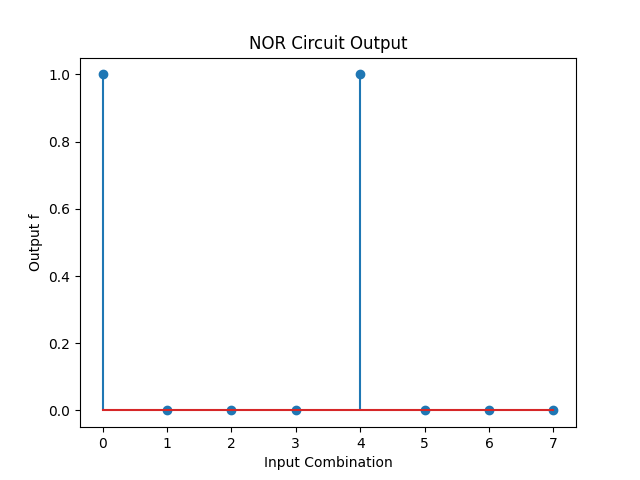
\includegraphics[width=10cm]{nor_graph.png}

\end{center}

\section*{Conclusion}

The Boolean expression of the circuit is:

$f = (Q + R)'$

\end{document}
